\chapter{Exercise 06}
\extitle{MyPlotLib}
\turnindir{ex06}
\exnumber{06}
\exfiles{MyPlotLib.py}
\exforbidden{None}
\makeheaderfilesforbidden

% ================================= %
\section*{Objective}
% --------------------------------- %
The goal of this exercise is to introduce you to plotting methods using different
libraries like Pandas, Matplotlib, Seaborn or Scipy.

% ================================= %
\section*{Instructions}
% --------------------------------- %
This exercise uses the following dataset: \texttt{athlete\_events.csv}\\
\\
Write a class called \texttt{MyPlotLib}. This class implements different plotting
methods, each of which takes two arguments:
\begin{itemize}
  \item a pandas.DataFrame which contains the dataset,
  \item a list of features names.
\end{itemize}

\hint{\href{https://towardsdatascience.com/feature-engineering-for-machine-learning-3a5e293a5114}{What is a feature?}}

\begin{itemize}
  \item \texttt{histogram(data, features)}: plots one histogram for each numerical feature in the list,
  \item \texttt{density(data, features)}: plots the density curve of each numerical feature in the list,
  \item \texttt{pair\_plot(data, features)}: plots a matrix of subplots (also called scatter plot matrix).
        On each subplot shows a scatter plot of one numerical variable against another one.
        The main diagonal of this matrix shows simple histograms.
  \item \texttt{box\_plot(data, features)}: displays a box plot for each numerical variable in the dataset.
\end{itemize}

% ================================= %
\section*{Examples}
% --------------------------------- %

\begin{figure}[h!]
  \begin{minipage}[l]{0.49\linewidth}
    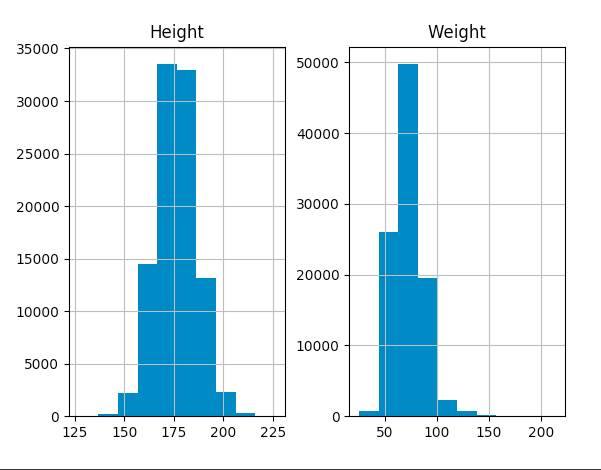
\includegraphics[scale=0.39]{assets/ex06_histogram.png}
    \caption{histogram}
  \end{minipage}
  \hfill
  \begin{minipage}[c]{0.49\linewidth}
    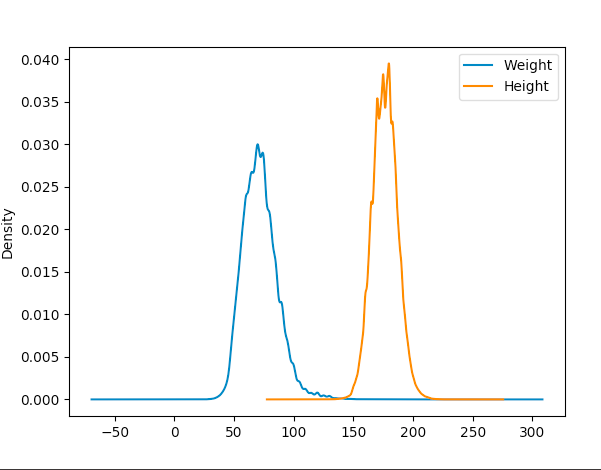
\includegraphics[scale=0.39]{assets/ex06_density.png}
    \caption{density}
  \end{minipage}
  
  \begin{minipage}[l]{0.49\linewidth}
    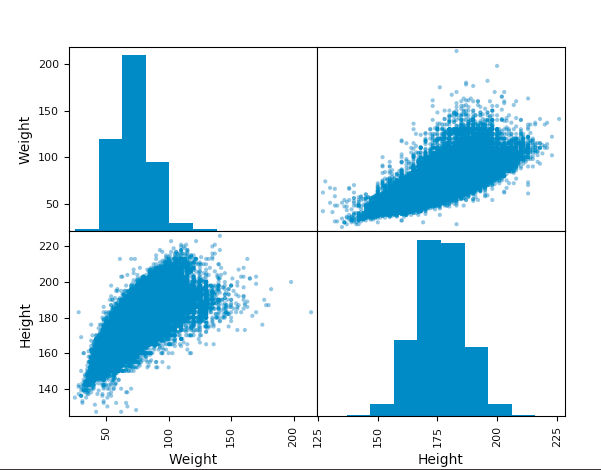
\includegraphics[scale=0.39]{assets/ex06_pair_plot.png}
    \caption{pair plot}
  \end{minipage}
  \hfill
  \begin{minipage}[c]{0.49\linewidth}
    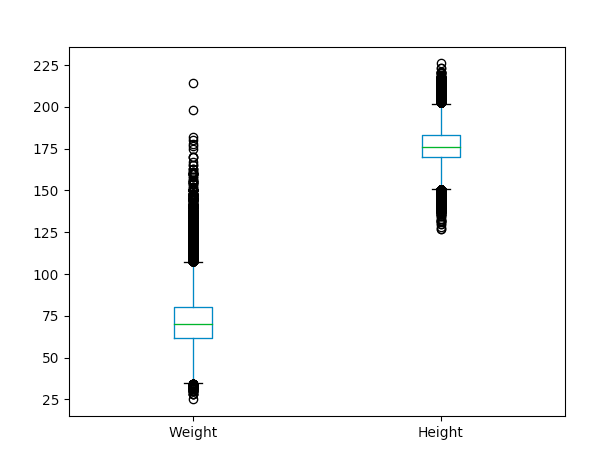
\includegraphics[scale=0.39]{assets/ex06_box_plot.png}
    \caption{box plot}
  \end{minipage}  
\end{figure}